%%%%%%%%%%%%%%%%%%%%%%%%%%%%%%%%%%%%%%%%%%%%%%%%%%%%%%%%%%%%%%%%%%%%%%%%%%%%%%%%%%%%%%%%%%%%%%%%%%%%
%%                                                                                                %%
%%                                                                                                %%
%%                                        MSc THESIS                                              %%
%%                                                                                                %%
%%                                                                                                %%
%%%%%%%%%%%%%%%%%%%%%%%%%%%%%%%%%%%%%%%%%%%%%%%%%%%%%%%%%%%%%%%%%%%%%%%%%%%%%%%%%%%%%%%%%%%%%%%%%%%%


%---------------------------------------------------------------------------------------------------
% PACKAGES & DOCUMENT CONFIGURATION
%---------------------------------------------------------------------------------------------------

\documentclass[a4paper]{article}
\usepackage[utf8]{inputenc} %setlength{parskip}{0.7em} usepackage{bibentry} nobibliography*
\usepackage[margin= 1.3in]{geometry}
\usepackage[colorinlistoftodos]{todonotes}
\usepackage{epigraph}
\usepackage{graphicx}
\usepackage{url}
\usepackage[nottoc]{tocbibind}
\usepackage{pgfgantt}
\usepackage{xcolor,colortbl}
\usepackage{pdfpages}
\usepackage{pdflscape}
\usepackage{rotating}
\usepackage{tikz}
\usepackage{svg}
\usepackage{amsmath}
 \usepackage[nottoc]{tocbibind}
 \usepackage{caption}
% \usepackage{hyperref}



\definecolor{Gray}{gray}{0.70}
\definecolor{LightCyan}{rgb}{0.88,1,1}

\newcolumntype{a}{>{\columncolor{Gray}}c}
\newcolumntype{b}{>{\columncolor{white}}c}


 % \usepackage[nottoc,numbib]{tocbibind}
% \usepackage{titlesec}
% %\titleformat{\chapter}[frame]{}{\thechapter}{0pt}{}
% \titleformat{\chapter}[display]
% {\normalfont\huge\bfseries}{\chaptertitlename\ \thechapter}{20pt}{\Huge}

% % this alters "before" spacing (the second length argument) to 0
% \titlespacing*{\chapter}{0pt}{0pt}{40pt}
\linespread{1.1}

\begin{document}

% \begin{center}\huge Synopsis of \textit{Making Mario Work Hard} par \Large Aaron Ceross (ac14580)
% \end{center}


%---------------------------------------------------------------------------------------------------
% TITLE PAGE
%---------------------------------------------------------------------------------------------------

\begin{titlepage}
    \begin{center}
        \vspace*{4cm}

        \Huge\textbf{Making Mario Work Hard}

        % \vspace{0.5cm}
        % Thesis Subtitle

        \vspace{2.5cm}

       \Large\textbf{Aaron Ceross}
       \\Supervisor: Dr. Benjamin Sach

        % \vfill
        \vspace{0.8cm}

        Work Plan\\
        COMSM2202 Research Skills

        \vspace{0.8cm}
        \vspace{0.8cm}

        % \includegraphics[width=0.4\textwidth]{university}

        % Department Name\\
        % University Name\\
        % Country\\
        \today

    \end{center}
\end{titlepage}


%---------------------------------------------------------------------------------------------------
% TABLE OF CONTENTS
%---------------------------------------------------------------------------------------------------

\tableofcontents

\pagebreak

%---------------------------------------------------------------------------------------------------
% CHP 1 --- EXECUTIVE SUMMARY
%---------------------------------------------------------------------------------------------------

\section{Executive Summary}

\subsection{Overview}

The aim of the proposed research project is to develop and implement software which visually
represents computational complexity through the video game medium. This `game engine' will be able
to graphically show user an NP-complete problem represented as a video game level as well as its
solution. An NP-complete problem is one with a solution that can be \textit{verified} quickly in
polynomial time, though an existing solution is not readily known or \textit{identifiable}
\cite{cook1984can}. It has been proven that certain classic video games, such as \textit{Super Mario
Bros} \cite{Aloupis2012}, are computationally hard in that the character could be made to solve an
arbitrary instance of a Boolean satisfiability problem (SAT). SAT is a type of NP-complete problem
in which the variables of the formula may be consistently replaced by the values TRUE or FALSE in a
way that the formula evaluates to TRUE, or `satisfiable' \cite{cook1971complexity}.

This research project is divided between 66\% Type I (software development) and 34\% Type II
(investigatory, research) and therefore more heavily centred on the development of the game engine
software. The project brings together multiple disciplines within computer science including
computer graphics, artificial intelligence as well as other fields including mathematics, and
ludology \cite{Hendrikx:2013:PCG:2422956.2422957}. The investigatory nature of the project evaluates
the computational complexity classes using different game level configuration and mechanics.

\subsection{Project goals}

In order to fulfil this aim, the research project will implement a game engine through achieving the
following objectives:

\begin{enumerate}

  \item Develop a platform game in which the mechanics are NP-complete; \vspace{-3mm}
  \item Develop a level generator which converts an instance of SAT into a playable level; \vspace{-3mm}
  \item Develop a visualisation of the SAT solving these levels by choosing a suitable path;   \vspace{-3mm}
  \item Evaluate level-generation and display of the SAT solver's decisions for efficiency and success against an
        established criteria or one developed during the project. \vspace{-3mm}

\end{enumerate}

\subsection{Methodology}

The project will design and develop the game engine according to the established theoretical
framework for video game NP-completeness within the relevant literature. As a means of verification,
the game engine should be able to produce the results produced in previous studies. Building upon
the established frameworks, the project will experiment with various approaches within content
generation in order to produce game levels that correctly implement the NP-complete elements of a
platform video game. These levels will be evaluated for their computational complexity and
`hardness'.

As the research is largely contingent on the development of robust software, the project will
utilise an Agile approach to the game engine development. The rapid development cycles are expected
to help quickly identify problematic areas and challenges.

\subsection{Expected project outcomes and added value}

The projected outcomes are multifaceted and wide-ranging. The immediate outcome is to allow
for further research within computer science and mathematics education on the feasibility and
efficiency of utilising the video game medium as a teaching aid. The successful completion of the
games engine also provides a possible tool for investigating the complexity of other games and
puzzles as it is generalisable and could be adapted to other complexity-testing frameworks.

% In addition, the research that will be conducted into computational complexity in conjunction with
% content generation may also be used to explore new methods for generating more difficult types of
% games which appeal to a broader range of users.

% The primary motivation of this research is to investigate the feasibility of the video game medium
% as a teaching tool to visualise and demonstrate concepts in computational complexity. This could be
% achieved through the evaluation of different instances of SAT in a video game setting.\@

% The aim of this project is to produce a game engine that is capable of visualising and demonstrating
% concepts in computational complexity through the evaluation of different instances of SAT.\@ The
% game engine would be able to take an instance of SAT and generate a human-playable level that is computationally hard. This level
% would then be able to be solved by a SAT solver. The solution to the level would then be visualised
% on screen.

\pagebreak
%---------------------------------------------------------------------------------------------------
% CHP 2 --- PROJECT PLAN
%---------------------------------------------------------------------------------------------------

\section{Expected Timeline}

\subsection{Overview}

This section addresses how the goals of the project will be determined as successfully completed.
The expected timeline for the project will run from 1 June --- 11 Sept 2015, approximately 15 weeks.
During this time, the project will pursue its task list, produce scheduled deliverables and reach
proposed milestones. The schedule and the interrelation of the work packages and associated
dependencies is further explained in Section 2.2.

\subsubsection{The dynamic nature of projects}

As with any project, there may be unforeseen changes made to the original work plan. This is not
necessarily a failure of the original work plan, but indication that the project recognises
developments within its own research as well as from others in the field. Therefore, this work plan
is to be viewed as an initial draft, which will be revisited often in order to reflect changes and
developments within the project.

\subsubsection{Project management structure}

In order to describe this project's management structure, it is necessary to re-articulate the
research goals and link the related work packages:

\begin{enumerate}

  \item Develop a platform game in which the mechanics of the game's level are NP-complete (Met by \textit{Work Package 2});
  \item Develop a visualisation of the SAT solving these levels by choosing a suitable path (Met by \textit{Work Package 3});
  \item Develop a level generator which converts an instance of SAT into a playable level (Met by \textit{Work Package 4});
  \item Evaluate level-generation and display of the SAT solver's decisions for efficiency and success against an
        established criteria or one developed during the project (Met by \textit{Work Package 5}).

\end{enumerate}

The project is divided into six \textit{work packages} that address each of the above project
goals. These work packages contain a number of related \textit{deliverables}. The completion of
certain deliverables and work packages represent \textit{milestones} in the project. The project is
considered successful if all the milestones are completed.

As mentioned in the executive summary, the project will implement an Agile methodology to the
software development. The rapid prototyping, modular, test-driven approach is hoped to developed a
robust game engine and quickly identify challenging areas of implementation. Figure~\ref{scrum}
below illustrates the envisaged development cycle. It is estimated that a single cycle
lasts no longer than seven days. Within a development cycle, the minimum functionality necessary for
continuation of the project should be completed. If the cycle is completed quickly (i.e. the
required functionality is achieved), the next development cycle begins. If there is a delay, the
next cycle maintains is allocated time period of a seven day maximum. This flexibility has been
incorporated into the schedule.

\begin{figure}[h!]

  \centering
    
\includegraphics[scale=0.25]{scrum}
  \caption{Agile development cyle.}
  \label{scrum}
\end{figure}

\subsection{Work Packages and Deliverables}

The work packages of the project represent key discrete areas of research and development during the
project's life-cycle. Each work package is defined by a set of tasks and contains a set of
deliverables, which are a means for verifying that the completion of those tasks. The work packages
for this project are as follows:

\begin{itemize}

  \item \textbf{Work Package 1: \textit{Foundational Work}}: This work package addresses the fundamental theoretical work of the project. Its deliverables include the literature review and project framework.     \vspace{-3mm}
  \item \textbf{Work Package 2: \textit{Core Game Engine Development}}: The game engine software in Work Package 2 provides the basis by which to represent computational complexity through a video game. The tasks in this work package will centre on implementing a game framework that is NP-complete according to available literature as well as provide the interfaces necessary for the completion of Work packages 3 and 4;          \vspace{-3mm}

  \item \textbf{Work Package 3: \textit{Engine Integration with SAT Solving Software}}: Work package
   3 focuses on integrating at least a single SAT solver into the game engine produced in
   Deliverable 2 in order to graphically visualise the solutions to the problem
   instances/levels;\vspace{-3mm}


\item \textbf{Work Package 4: \textit{Level Generation}}: This part of the project addresses the generation of large scale levels beyond those generally found within 2D platform games.\vspace{-3mm}
  \item \textbf{Work Package 5: \textit{Experiments and Data Collection}}: This deliverable utilises the developed game engine to examine different classes of complexity (e.g. PSPACE-hard) through the modification of framework and utilising the large-scale level generation of Work Package 4.\vspace{-3mm}
  \item \textbf{Work Package 6: \textit{Project Evaluation and Thesis Write-up}}: This is the final deliverable which evaluates the progress of the project, highlighting significant findings. Work Package 6 includes the thesis and posters as deliverables. This work package spans the course of the entire project.


\end{itemize}

\noindent Each work package will be considered individually with an explanation of each of the proposed
deliverables. The specific tasks will inevitably change based on the challenges that arise during
the development of each deliverable. For this reason, only deliverables are contained within this
document. The work packages and the related deliverables are illustrated in a Gantt chart (See section
2.4).

\subsubsection{Work Package 1 --- Foundational Work}

This deliverable relates to the preliminary work that has been conducted during the Research Skills
module (COMSM2202) Research Skills module.  The deliverables for this work package have been
completed at the time of this work plan's submission  as shown in Table~\ref{WP1}. As such, these
have not been included in the Gantt chart. However, it will be noted that the project is in constant
evolution and future findings may require that certain elements of this work package may need to be
altered. For example, the literature list and research review will largely inform the literature
review of the final thesis. Therefore, these deliverables will most certainly continue to be
revised.

\begin{center}
\captionof{table}{Work Package 1 Deliverables}
    \begin{tabular}{ | l | l | l |}
    \hline
    \rowcolor{Gray}
    Deliverable Number & Deliverable & Deadline \\ \hline

    D.1.1. & Synopsis & 20 February 2015 \\ \hline

    D.1.2. & Literature List & 06 March 2015 \\ \hline

    D.1.3. & Research Review & 05 May 2015 \\ \hline

    D.1.4. & Work Plan & 11 May 2015 \\ \hline


    \end{tabular}

\label{WP1}
\end{center}

\subsubsection{Work Package 2 --- Core Game Engine Development}

Work package 2 represents the start of the software development within the project. The deliverables
within this work package establish the basis from which to. While this is a technically focused work
package, it incorporates investigatory elements.

The first deliverable of Work Package 2 is the initial prototype (D.2.1). This deliverable
establishes a proof of concept software that shows a the solution to a maze using depth-first
recursion. The graphical output should only identify the correct solution, even if the solver
explores different paths.

Deliverable 2.2 provides the 2D platform game environment. This will include a player sprite,
collision, enemies, and basic physics (for jumping and falling). Within this deliverable the tasks are:

\begin{itemize}

  \item Develop a player class;
  \item Establish player controls;
  \item Implement simple player sprite animation;
  \item Establish rules of collision;
  \item Simple graphics to emulate 2D platform game style;

\end{itemize}

The next deliverable, 2.3, focuses on the development of the elements in a game level that make a
game NP-complete. These level elements include variable gadgets and clauses, which correspond to
clauses within a Boolean formula. This deliverable will make extensive use of the frameworks
established in literature.

Completion of this work package is provided by D.2.4, Software Unit Testing Results. The modules in
the game engine will be unit tested for correctness and to address any software bugs. Testing will
occur through out the development process, but a small amount of time is dedicated at the end of the
work package for specific testing. Play testing and graphics testing are also included in this
deliverable.  Documentation of all the design decisions and tests are addressed in Work Package 6,
Deliverable 6.1, Technical Report on Game Engine Design.

% Develop platform game modules
% - player class
% - collision
% - level map - this will be based on the framework provided by Aloupis
% - variable gadgets
% - clauses
% - start and end gadget
% - unit and play testing

% \begin{center}
%     \begin{tabular}{ | l | l | l |}
%     \hline
%     \rowcolor{Gray}
%     Deliverable Number & Deliverable & Deadline \\ \hline

%     % D.2 & Platform Game Development &  \\ \hline

%     D.2.1. & Initial Prototype & 30 May 2015. \\ \hline

%     D.2.2. & Platform Game Prototype & 10 June 2015 \\ \hline

%     D.2.3. & Playable Level based on NP-complete problem & 22 June 2015 \\ \hline

%     D.2.4. & Software Unit Testing Results & 25 June 2015 \\ \hline

%     \hline
%     \end{tabular}
% \end{center}

% Work has already commences on this work package, ahead of the proposed schedule. A more detailed
% explananation is provided in SECTION SOMETHING.


\subsubsection{Work Package 3 --- Engine Integration with SAT Solving Software}

During this work package, the project's focus is to integrate the completed game engine and
integrate it with a SAT solver. The research review had identified a number of eligible solvers. To
begin, Deliverable 3.1 surveys the individual SAT solvers, looking at the source code and
evaluating the ease with which the solver can be integrated into the engine.

There are a number of different solvers to evaluate, each with differing qualities. These include:
\texttt{zChaff} \cite{fu2004zchaff}, \texttt{Sato} \cite{zhang1997sato}, and \texttt{MiniSAT}
\cite{sorensson2005minisat}. Once a suitable solver has been identified, its decisions will be mapped
to the game character animations and level position movements within the game engine. There is scope
to be able to integrate multiple SAT solvers and run simultaneous instances. This possibility will
be explored during the course of Work Package 3.

This work package concludes with further tests (D.3.3) to ensure that the
major integration challenges and bugs have been addressed and rectified.

% \begin{center}
%     \begin{tabular}{ | l | l | l |}
%     \hline
%     \rowcolor{Gray}
%     Deliverable Number & Deliverable & Deadline \\ \hline

%     D.3.1. & Technical Analysis of SAT Solvers & 03 July 2015. \\ \hline

%     D.3.2. & Integration & 13 July 2015 \\ \hline

%     D.3.3. & Unit Tests & 15 July 2015 \\ \hline

%     \hline
%     \end{tabular}
% \end{center}

\subsubsection{Work Package 4 --- Level Generation}

A game level within the game engine is merely a SAT problem instance. Therefore, this work package
incorporates means by which to specify the types of SAT problem instances that may be solved by the
game engine. Deliverable 4.1 concerns the basic level generation algorithm, which will most likely
use a `chunk'-based approach to generation \cite{mawhorter2010procedural}. Within this approach,
pre-determined gadgets will be created and the generation algorithm will tie these together,
according to the specified input.

The level generation will require specific constraint against being able to solve the level without
generating a satisfying assignment for the SAT instance. If this is possible, then the level
instance is not guaranteed to be NP-complete and is a significant feature gap in the software.
Therefore, one of the more significant tasks of this deliverable is to test for the existence of
robust cross-over gadgets, which would prevent the player character from avoiding certain variable
gadgets and clauses.

The view module (Deliverable 4.2) will allow for the game view window to `zoom out' in order for the
user to adequately see the path of the game character in solving a large level. The View Module may
also include a `speed-up' mechanism for such levels. This will be investigated during the
implementation and if it is felt to add to the user experience.  A stable version will be produced
with a hard-coded tested level prior to engaging in the next task: development of large scale
levels.

Large scale levels are necessary insofar as these may provide means for visualising other classes of
complexity. For D.4.3, these may be generated in a deterministic manner, within a set of constraints
such that the game gadgets are composed in a manner ensuring NP-completeness. There may be a
possibility that the levels will be tested on high powered computers in order to assess the
robustness of the generation method.

% \begin{center}
%     \begin{tabular}{ | l | l | l |}
%     \hline
%     \rowcolor{Gray}
%     Deliverable Number & Deliverable & Deadline \\ \hline


%     D.4.1. & Procedural level generation & 30 July 2015. \\ \hline

%     D.4.2. & View Module & 02 August 2015 \\ \hline

%     D.4.3. & Scale-Testing Results & 28 August 2015 \\ \hline

%     \hline
%     \end{tabular}
% \end{center}

\subsubsection{Work Package 5 --- Experiments with Complexity Classes}

This work package is dedicated to examining different frameworks for testing the complexity of 2D
platform video games. Building on the models found in literature, such as Aloupis \textit{et al}.
\cite{Aloupis2012}, the deliverables will critically examine and perhaps even extend the proposed
models.

In Deliverable 5.1, a series of tests and experiments will be constructed for the game engine. The
main experiment will to determine which SAT-instances are harder for the SAT-solver. This will be
done with various reductions of SAT. The results will be measured for efficiency and time. These
tests and experiments may also help in devising test for describing different classes of
computational complexity in video games aside from NP-complete. This may include PSPACE-hard, as
literature, particularly Fori\v{s}ek, has suggested that certain 2D platform games fall within this
classification \@\cite{DBLP:conf/fun/Forisek10}.

The further software developments needed to implement these are documented and described in
Deliverable 5.2. This may include integrating a True quantified Boolean formula (TQBF) solver into
the existing engine for PSPACE-hard levels. A TQBF-solver utilises the same recursive solving
strategy as a SAT-solver and as a consequence may be quicker to implement into the engine.


\subsubsection{Work Package 6 --- Project Evaluation and Thesis Write-up}

This work package is comprised of tasks relating to the reporting, analysis and evaluation of the
project. Importantly, this work package includes the write-up of the thesis. As such, Work Package 6
receives input from all other work packages upon their completion. The deliverables are reports
which may either be technical reports, which document the software development process or
experimental reports, which are concerned with exploring unresearched areas within the project (e.g.
level generation and scaling of SAT instances). In all deliverables with this work package, existing
literature will be constantly evaluated and surveyed.

The design of this work package is to ensure that the thesis is constantly in a state of development
throughout the life-cycle of the project. This work package achieves this by dividing the thesis
elements into write-ups of the various work packages, detailing the theoretical background,
implementation decisions, outcomes, and evaluation. This can be seen in the project's Gantt chart in
Section 2.4. This work plan actively avoids leaving too little time at the end to fully articulate
and detail the findings of this project.

The first two deliverables D.6.1 and D.6.2 are technical reports documenting the development of the
game engine as well as highlighting any novelty and issues that have not been previously addressed
within the literature. In D.6.1, the results of WP 2 are detailed and summarised, taking its input
from. The developed software will be evaluated against the frameworks established within existing
research literature. In D.6.2, the focus is on SAT solvers and their functionality. The report will
detail which SAT solver(s) had been chosen as well as the features. This feature list will also
inform the experimental set-up of D.5.1.

The next two deliverables of this work package focus more strongly on the experimental and
investigatory nature of the project. Deliverable 6.3 centres on the developing and implementation of
a heuristic method for generating quality levels (i.e. graphical representation of SAT problem
instances). The primary focus is to develop a consistent and efficient method using a chunk-based
approach.

The most experimental and investigatory deliverable, D.6.4, is writes up the data-collection and
analysis from D.5.1, described above. The report will detail the experimental set-up and evaluation
criteria. This criteria will be determined from literature that is available at the time of the
experiments.

The latter two deliverables concern the poster and submission of the final thesis. As stated above,
the construction of this work package has been devised so that the overall thesis has been being
written consistently and throughout the project.

% \begin{center}
%     \begin{tabular}{ | l | p{5cm} | l |}
%     \hline
%     \rowcolor{Gray}
%     Deliverable Numbler & Deliverable & Deadline \\ \hline

%     D.6.1. & Technical Report on Game Engine Design & 25 June 2015. \\ \hline

%     D.6.2. & Technical Report on SAT Solver Integration & 15 July 2015 \\ \hline

%     D.6.3. & Level Generation Results and Analysis Report & 30 July 2015 \\ \hline

%     D.6.4. & Experimentation with Differing Complexity Tests Results and Analysis Report & 06 September 2015 \\ \hline

%     D.6.5. & Poster & DATE \\ \hline

%     D.6.6. & Thesis Submission & DATE \\ \hline

%     \hline
%     \end{tabular}
% \end{center}
\pagebreak

\subsubsection{List and schedule of Deliverables}

The full list of deliverables are provided in Table~\ref{deliverables}.

\begin{center}
\captionof{table}{Table of Deliverables}
    \begin{tabular}{ | l | p{5cm} | l |}
    \hline

    \rowcolor{Gray}

    \multicolumn{3}{|c|}{\textbf{Work Package 1}} \\ \hline

    Deliverable Number & Deliverable & Deadline \\ \hline

    D.1.1. & Synopsis & 20 February 2015 \\ \hline

    D.1.2. & Literature List & 06 March 2015 \\ \hline

    D.1.3. & Research Review & 05 May 2015 \\ \hline

    D.1.4. & Work Plan & 11 May 2015 \\ \hline

    \rowcolor{Gray}

    \multicolumn{3}{|c|}{\textbf{Work Package 2}} \\ \hline

    D.2.1. & Initial Prototype & 30 May 2015 \\ \hline

    D.2.2. & Platform Game Prototype & 10 June 2015 \\ \hline

    D.2.3. & Playable Level based on NP-complete problem & 22 June 2015 \\ \hline

    D.2.4. & Software Unit Testing Results & 25 June 2015 \\ \hline


    \rowcolor{Gray}

    \multicolumn{3}{|c|}{\textbf{Work Package 3}} \\ \hline


    D.3.1. & Technical Analysis of SAT Solvers & 01 July 2015 \\ \hline

    D.3.2. & Integration & 08 July 2015 \\ \hline

    D.3.3. & Unit Tests & 10 July 2015 \\ \hline


    \rowcolor{Gray}

    \multicolumn{3}{|c|}{\textbf{Work Package 4}} \\ \hline

    % Deliverable Number & Deliverable & Deadline \\ \hline


    D.4.1. & Procedural Level Generation & 22 July 2015 \\ \hline

    D.4.2. & View Module & 29 July 2015 \\ \hline

    D.4.3. & Scale-Testing Results & 05 August 2015 \\ \hline

    D.4.4. & Integration with Game Engine & 07 August 2015 \\ \hline

    \rowcolor{Gray}

    \multicolumn{3}{|c|}{\textbf{Work Package 5}} \\ \hline

    % Deliverable Number & Deliverable & Deadline \\ \hline


    D.5.1. & Complexity class Experiments & 19 August 2015 \\ \hline

    D.5.2. & Game Engine Updates & 26 August 2015 \\ \hline


    \rowcolor{Gray}

    \multicolumn{3}{|c|}{\textbf{Work Package 6}} \\ \hline

    % Deliverable Numbler & Deliverable & Deadline \\ \hline

    D.6.1. & Technical Report on Game Engine Design & 10 June 2015 \\ \hline

    D.6.2. & Technical Report on SAT Solver Integration & 17 July 2015 \\ \hline

    D.6.3. & Level Generation Results and Analysis Report & 14 August 2015 \\ \hline

    D.6.4. & Experimentation with Differing Complexity Tests Results and Analysis Report & 26 August 2015 \\ \hline

    D.6.5. & Poster & TBD \\ \hline

    D.6.6. & Thesis Submission & 11 September 2015 (provisional) \\ \hline

    %\hline
    \end{tabular}
    \label{deliverables}
\end{center}
\pagebreak
\subsection{Milestones}

Milestones represent the completion of significant stages within the project; these stages re-
establish the baseline of the project. Each milestone is verified by the completion of deliverables.
This project has four milestones, roughly corresponding to three to four weeks each. A full table
table of milestones is illustrated in Table~\ref{milestones}. The interrelation between milestones and work packages is shown in Figure~\ref{org}.

\begin{itemize}

  \item \textbf{M.1: \textit{Completion of Game Engine}}: The complete game engine includes the 2D platform level mechanics (D.2.1);
\vspace{-3mm}
  \item \textbf{M.2: \textit{Completion of Level Generation Modules}}: The second milestone is to successfully
  integrate the software modules for level generation. This corresponds to the research and
  development in Work Package 4 as well as the analysis produced in D.6.3 in Work Package 6;
\vspace{-3mm}
  \item \textbf{M.3: \textit{Completion of Experiments and Engine Update}}: The third milestone is
the successful completion of complexity experiments in Work Package 5. The results are hoped to
provide any improvements and updates for the game engine. This represents the last major additions
to the engine and therefore closes major development.
\vspace{-3mm}
\item \textbf{M.4: \textit{Submission of Thesis}}: The final milestone is the submission of the MSc
thesis, which represents the end of the project. The development of the thesis will have been on-
going through out the project as well as during the specific time allocated for final write-up.
\vspace{-3mm}

\end{itemize}

\begin{center}
\captionof{table}{Table of Milestones}
    \begin{tabular}{ | p{1.2cm}  | p{6.2cm} | p{4cm} | p{3cm} |}
    \hline
    \rowcolor{Gray}
    Number & Milestone & Verification & Expected Date \\ \hline

    M.1. & Completion of Game Engine & D.2.2, D.2.3, D.2.4, D.3.2, D.6.1, D.6.2 & 25 June 2015. \\ \hline

    M.2. & Completion of Level Generation Modules & D.4.1, D.4.2, D.4.3, D.6.3 & 30 July 2015 \\ \hline

    M.3. & Completion of Experiments and Engine Update & D.5.1, D.5.2, D.6.4 & 30 July 2015 \\ \hline

    M.4. & Submission of Thesis & D.6.6 & 11 September 2015 \\ \hline

    \hline
    \end{tabular}
    \label{milestones}
\end{center}

\begin{figure}[htbp]
  \centering
  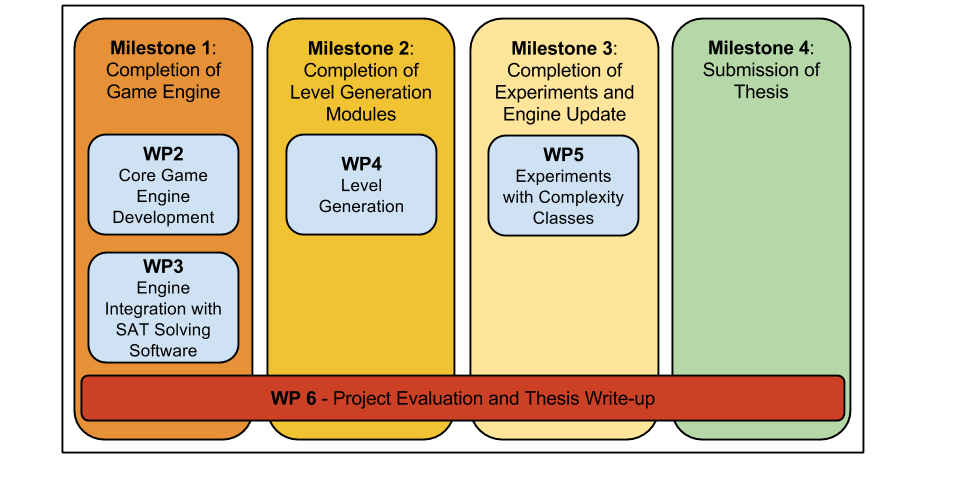
\includegraphics[scale=0.4]{organisation(1)}
  \vspace{-3mm}
  \caption{Interrelation between Milestones and Work Packages}
  \label{org}
\end{figure}


\pagebreak

\begin{landscape}
\subsection{Gantt Chart}
% Figure~\ref{Gantt} depicts the Gantt chart for the research project, which may be altered according to development.
% \begin{figure}[htbp]
%   \centering
%   \includesvg{gantt.svg}
%   \caption{svg image}
% \end{figure}




% 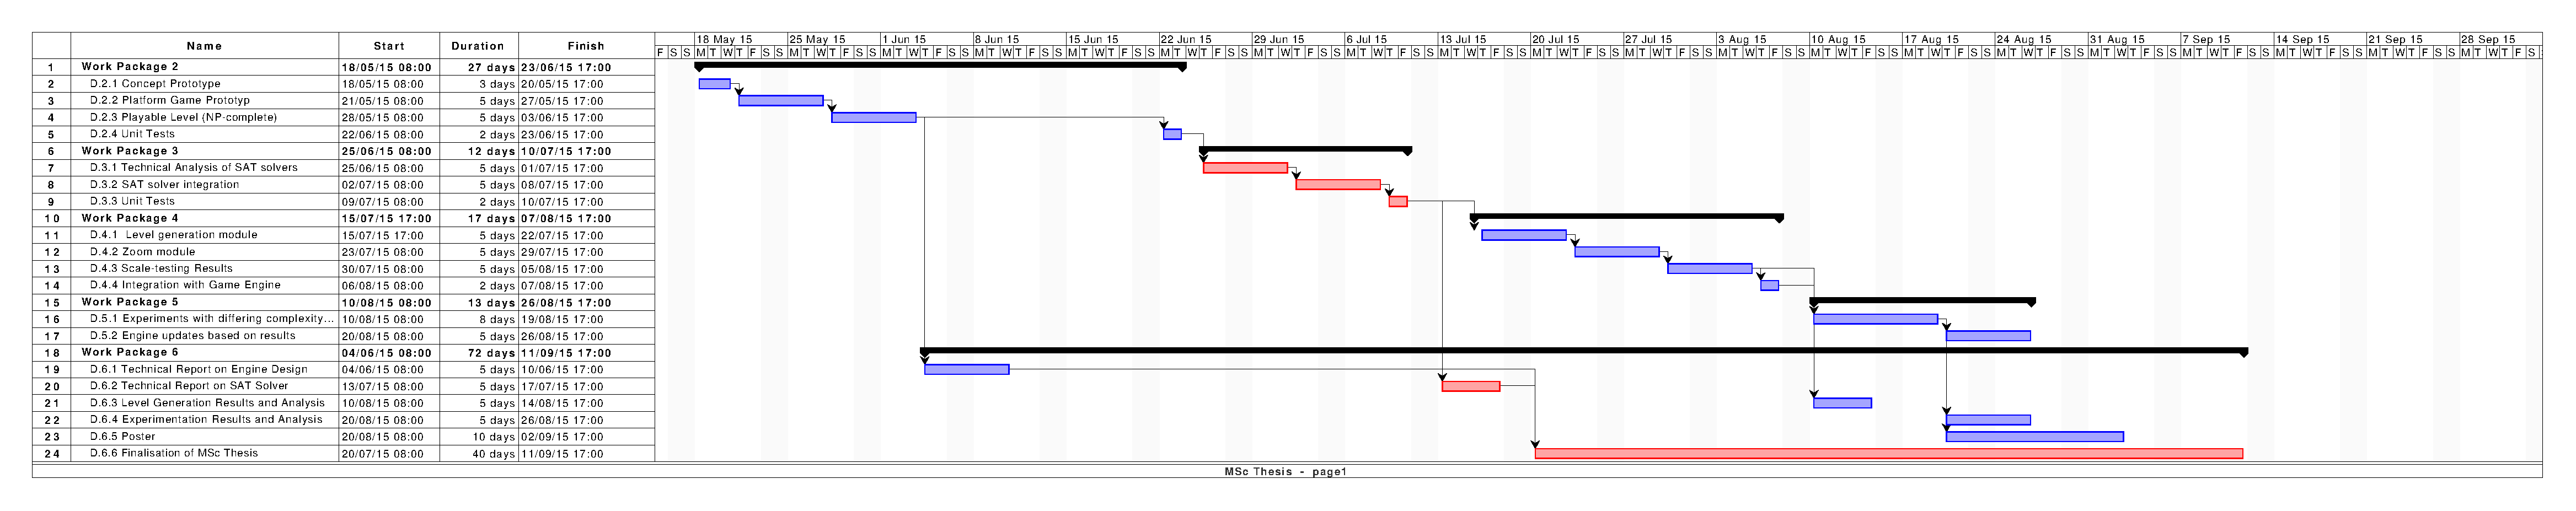
\includepdf[pages={1}]{gantt.pdf}


% \begin{sidewaysfigure}
    % \centering
    % \begin{tikzpicture}[scale=5]
    %      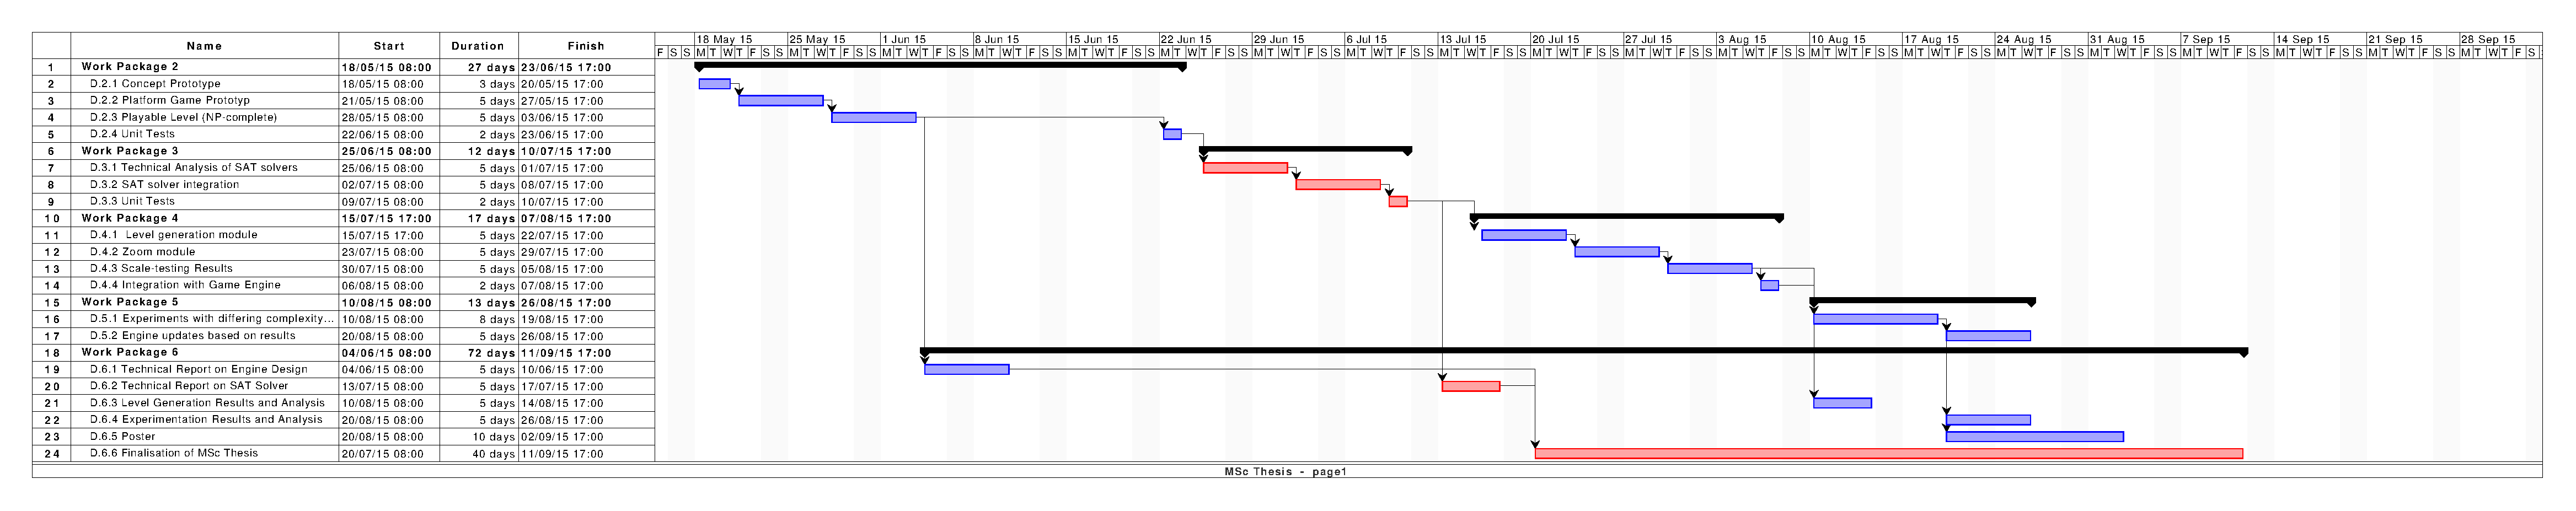
\includegraphics[scale=0.40]{gantt}
    % \end{tikzpicture}
    % % \caption{Box plot of number of positions sent per iteration using this scheme}
    % \label{fig:awesome_image}
% \end{sidewaysfigure}

\begin{figure}[h]

  \centering
  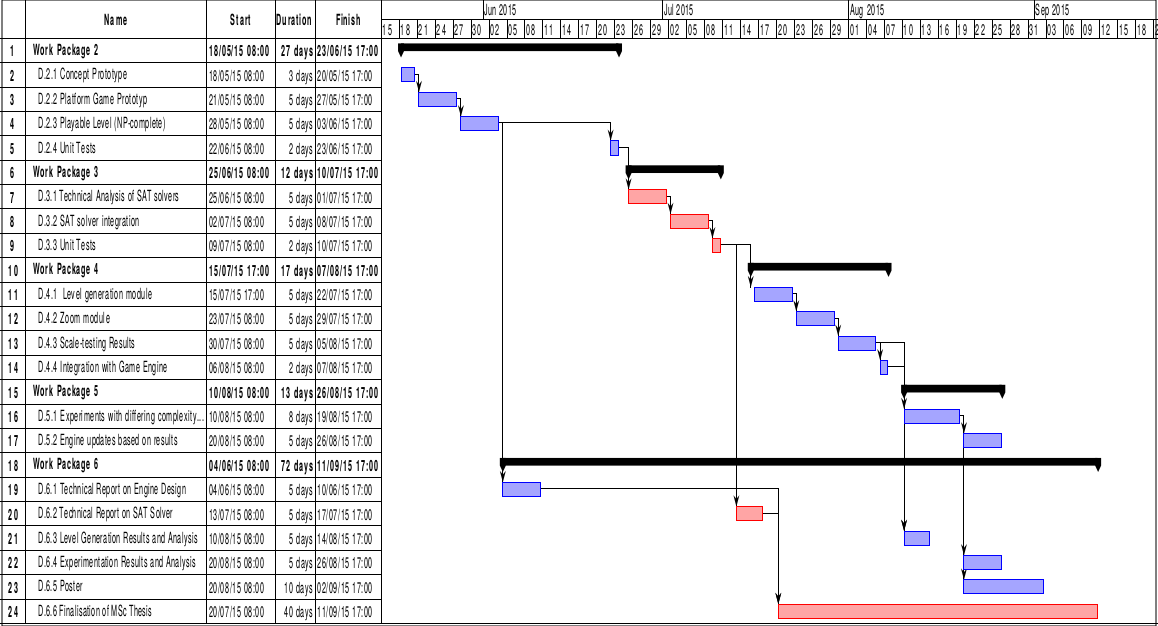
\includegraphics[trim=0cm 0cm 0.0cm 0.0cm, clip=true, width=9in,height=4.25in, angle=0]{gantt2}
    %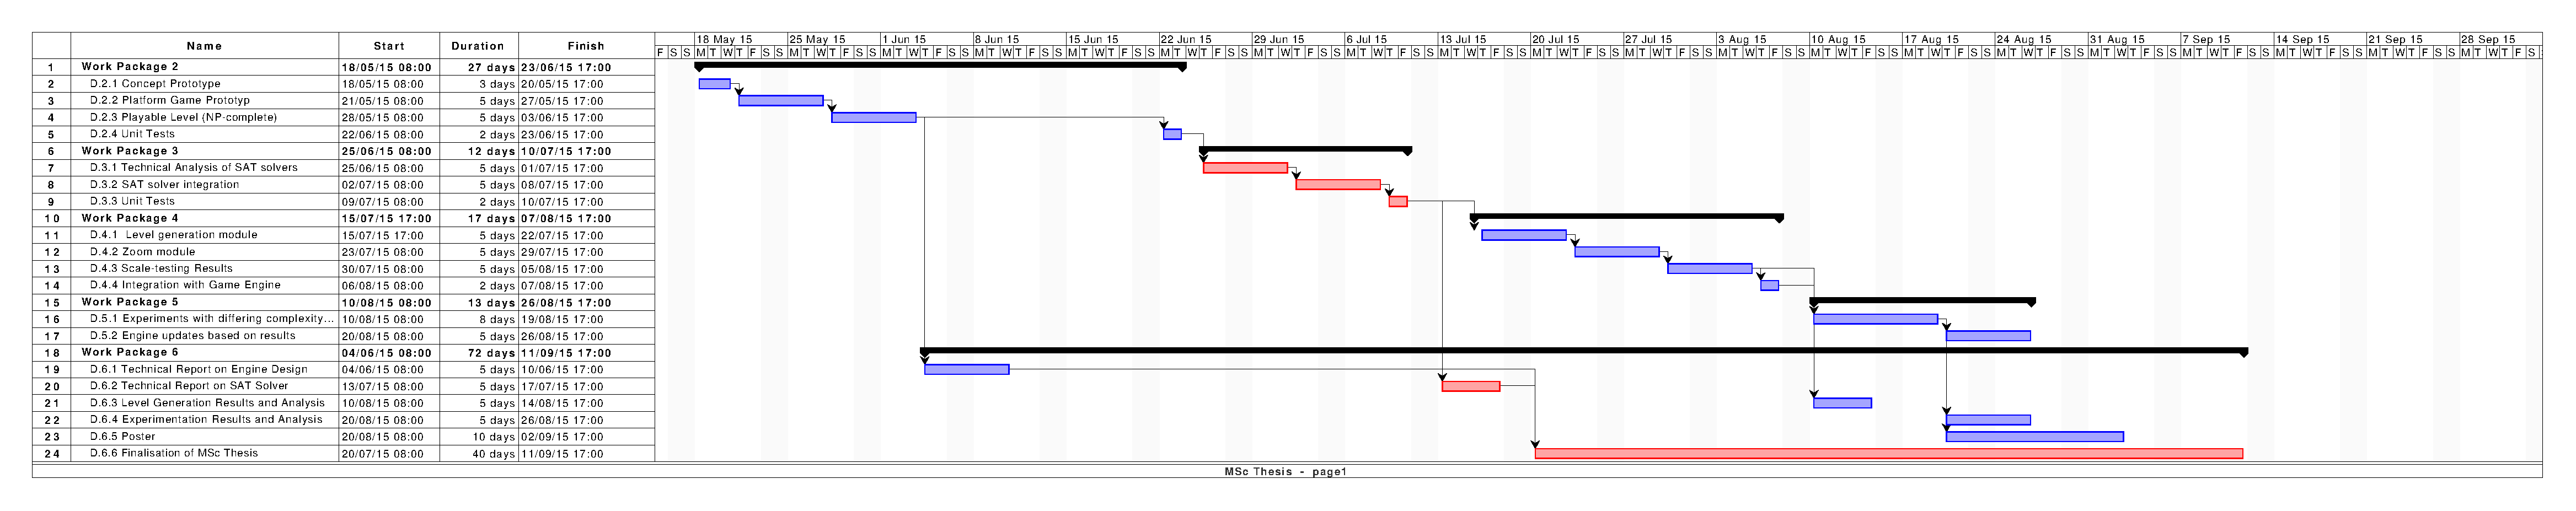
\includegraphics[scale=0.35]{gantt}
  % \caption{Reseach project's Gantt chart}
  \label{Gantt}
\end{figure}
\pagebreak
\end{landscape}

%---------------------------------------------------------------------------------------------------
% CHP 2 --- TIME LINE
%---------------------------------------------------------------------------------------------------


% This document and all the tables and schedules contained herein will be continually updated
% throughout the lifecycle of the project at review periods. For the initial development cycle, the
% following



% Establish success criteria

% Develop platform game modules
% - player class
% - collision
% - level map - this will be based on the framework provided by Aloupis
% - variable gadgets
% - clauses
% - start and end gadget
% - unit and play testing

% Re-evaluate criteria

% Interaction with SAT
% - use of zChaff and MiniSAT
% - how to interpret SAT decisions as player actions
% - represent decisions visually
%   - this can be achieved through only printing the actions where the solution exists.


% Re-evaluate criteria

% Level generation module
% - input of SAT reduction
% - pick from list
% - input formula
% - test large scale levels

% Write up


%---------------------------------------------------------------------------------------------------
% CHP 1 --- RISK ANALYSIS
%---------------------------------------------------------------------------------------------------

\section{Risk analysis and contingency plan}


\subsection{Risk assessment methodology}

The risks need to be assessed in order to identify which risks can most impact the progress of the
project and whether there is an available contingency. In order to prioritise, the risks are ranked
according to probability and impact. Likelihood and severity may either be assigned a value from 1
to 5:

\begin{enumerate}

  \item Very Low;
  \item Low;
  \item Medium;
  \item High;
  \item Very High.

\end{enumerate}

\noindent The two values are combined: \textit{Likelihood} + \textit{Severity} giving a total possible
score of ten (10), which is the risks quantified impact.
% \centerline{\textit{Likelihood X Perceived Impact --- Likelihood of Contingency X Perceived Impact}}
\subsection{Table of Risks and Contingencies}

Table~\ref{risk} identifies the risks associated with this project.

\begin{center}
\captionof{table}{Table of Risks}
    \begin{tabular}{ | p{4.2cm} | l | p{2.1cm} | p{1.1cm} | p{5cm} |}
    \hline
    \rowcolor{Gray}
    Risk & Likelihood & Severity & Impact & Contingency Plan \\ \hline


    % Personal illness/injury & Low & Low to Very High & The contingency action would depend on the
    % type of illness. For example, mild illness/injury may require minor adjustment in schedule,
    % reducing the pace of development. Severe illness and injury would be immediately reported to
    % supervisor and the university. Future plans would be decided in conjunction with supervisor and
    % university  \\ \hline

    SAT solver decisions too fast for appropriate graphical display & Medium & Very Low & 4 &
    The display may have a delay in order to ensure the decisions are not displayed too fast. \\ \hline

    SAT solver decisions too slow for appropriate graphical display & Medium & Low & 5 &
    Decisions may be put into a stack or linked-list and then displayed at an appropriate speed. \\ \hline

    Difficulty in visualising SAT decisions as video game movements & Medium & Medium & 6 & Remove
    animations and simplify 2D platform game mechanics. If the delay becomes too severe, the game may
    be simplified into a maze. \\ \hline

Available computing power does not manage large scale levels & High & Medium & 7 & Request use
of university's HPC facilities (e.g. BlueCrystal) in order to test game engine capabilities. \\
\hline

Levels do not generate according to rules & High & Medium & 7 & Hard-code level according to established framework. \\ \hline


    SAT does not integrate with the game engine & Medium & Very High & 8 & Reduce capability into a simple depth-first search maze solver and design a SAT instance as a maze.
    \\ \hline




    \hline


    \end{tabular}
    \label{risk}
\end{center}

\noindent \textbf{Note on personal illness} \\

\noindent Personal illness has been separated from the other identified risks as it is a risk of
which the impact may be low or very high, depending on the circumstances. Personal illness or injury
is constant risk of life and therefore, the contingency action would depend on the type of illness.
For example, mild illness/injury may require minor adjustment in schedule, reducing the pace of
development. Severe illness and injury would be immediately reported to the supervisor and the
university. Future plans would be decided in conjunction with supervisor and  university.

\subsubsection{Managing high impact risks}

This section address the risks with the highest impact (score 7 and over). The effects of these
risks would fundamentally alter the structure and outcome of the research project. This section
explains the contingencies in more detail and the possible direction the project may take. \\
\\
\noindent \textbf{Failure to generate level according to rules} \\

\noindent Failure to generate the levels according to user input or algorithm represents an
investigatory risk. Procedural content generation is described in its own literature as very
challenging and it is likely that generating levels with the desired quality may prove quite
difficult. The difficulty represents a research outcome in and of itself, but one of the core
research aims is to have levels that represent SAT instances. The contingency plan would be to
`hard-code' levels onto a map according to the established NP-complete frameworks recognised in
previous research. This would allow for the project to meet its aims without significant compromise.\\

\noindent \textbf{Failure to integrate SAT solver}\\

\noindent This represents a significant risk as use of a SAT solver is a vital feature. Should
integrating a SAT solver into the game engine prove significantly difficult, the game engine may be
reduced to a maze solver. A maze would incorporate the necessary features to prove NP-completeness.
The maze would then be solved with a basic depth-first recursive function. This has already been
achieved in a prototype (see section 4 below). While not ideal, it does allow for the project to
develop a visualisation tool for demonstrating complexity. \\

\noindent \textbf{Available computing power does not manage large scale levels} \\

\noindent Development work will be carried out primarily on a laptop, which has obvious
computational limitations. In the event that this becomes a factor restricting development. The work
on the level generation may be moved to the computer facilities provided by the university (e.g the
computer labs in Merchant Ventures Building). Should further computational power be necessary, the
university's high powered computing (HPC) facility (i.e. BlueCrystal) may be approached. If this is
not possible, the generation of very large levels may be omitted. This will have an effect on the
experimentation with complexity classes (Work Package 5). The solution is to be in contact with
those in the HPC early and consistently in order to book time.

\pagebreak
%---------------------------------------------------------------------------------------------------
% Current Progress
%---------------------------------------------------------------------------------------------------

\section{Significant progress made towards the project}

\subsection{Preliminary prototype}

During the research view and the creation of this work plan document, work had begun on Deliverable
2.1, which produces a very simplified prototype of a maze puzzle and a recursive depth- first
solver. The goal of the prototype is to establish the means and methods for recursive solver and its
graphical output. The current prototype has been written in C++ and utilises Simple DirectMedia
Layer (SDL)\footnote{https://www.libsdl.org} for graphics. SDL has been chosen as it is a very
extensive library that has been used in conjunction with C++ to produce games.

In the initial prototype, a maze has been drawn in a text file and read into the program. The
program contains rules for valid moves, thereby preventing the solver from going through walls. The
solver utilises a recursive depth-first search in order to find the exit of the maze (see
Figure~\ref{prototype} for an illustration).\footnote{A video of the prototype can also be viewed
at: \url{ https://youtu.be/4fm5DUeyGAE}} This recursive search is similar to the recursive DPLL
algorithm used in many SAT solvers \cite{zhang2002quest,gomes2008satisfiability}. The prototype
therefore has been useful in order to understand how to link the solver's branching decisions with
the graphics library.

\begin{figure}[h!]

  \centering
    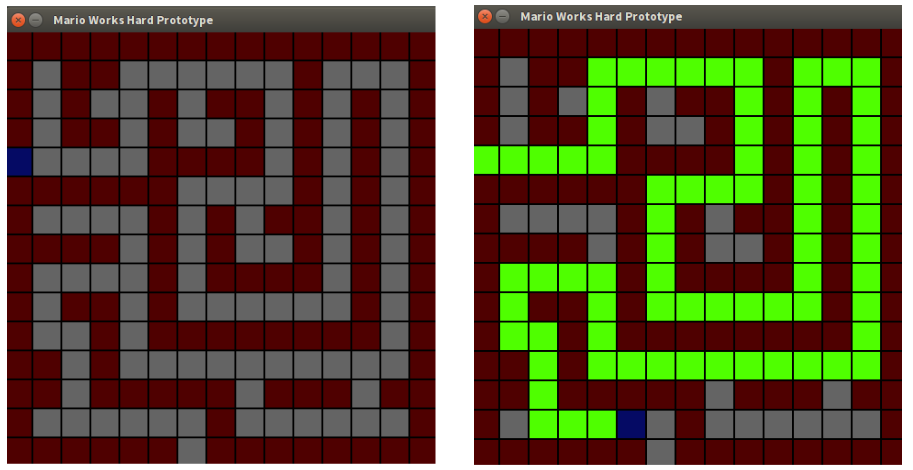
\includegraphics[scale=0.35]{compare}
  \caption{Screenshot of the prototype depth-first recursive maze solver. In the maze, red represents walls, grey for empty space, blue for the solver's current position and green for the solution path. The left image shows the start, with the maze unsolved. The right image shows the path to solve the maze. Only the correct solution path is displayed and not every branching decision.}
  \label{prototype}
\end{figure}

The initial prototype is encouraging and has given the project a strong start to exploring the next
areas of research and development. The next stages are to convert the maze into a generic 2D
platform level and develop the player character class (i.e. a `Mario'-like figure), introduce
collision, and other level elements, pursuing the goals of Deliverable 2.2 and 2.3.

\subsection{Future Work}

The immediate future work of the project is to complete the first iteration of the game engine
prototype using the encouraging results from the initial prototype. Further literature review is
also necessary in order to supplement current knowledge of video game variable gadgets, in order to
better translate these into the game engine.

%
% \begin{figure}[h!]

%   \centering
%     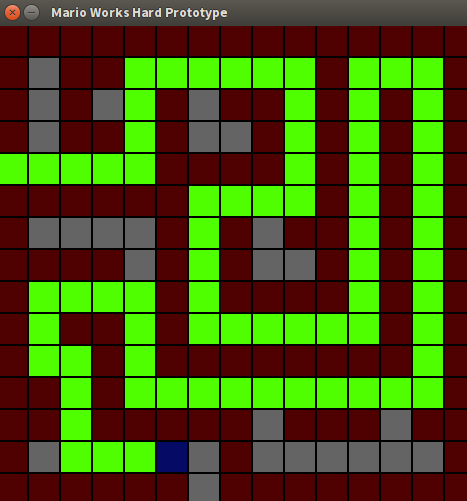
\includegraphics[scale=0.45]{proto2}
%   \caption{Graphical output of depth-first recursive maze solver. Only the solution path is displayed (tiles in green) and not every branching decision.}
%   \label{proto2}
% \end{figure}


% \end{document}

\pagebreak

%---------------------------------------------------------------------------------------------------
% BIBLIOGRAPHY
%---------------------------------------------------------------------------------------------------

\bibliographystyle{abbrv}
\bibliography{references.bib}

\end{document}
